\section{Datos y metodología}
\label{sec:metodologia}

Todas las decisiones de esta sección se fijaron en un plan de análisis escrito antes de la estimación principal; los
cambios posteriores, con su fecha y su motivo, están en la bitácora del plan (Anexo~\ref{sec:anexo-plan}).

\subsection{Proceso, fuentes y unión}
\label{sec:datos}

\begin{figure*}[t]
\centering
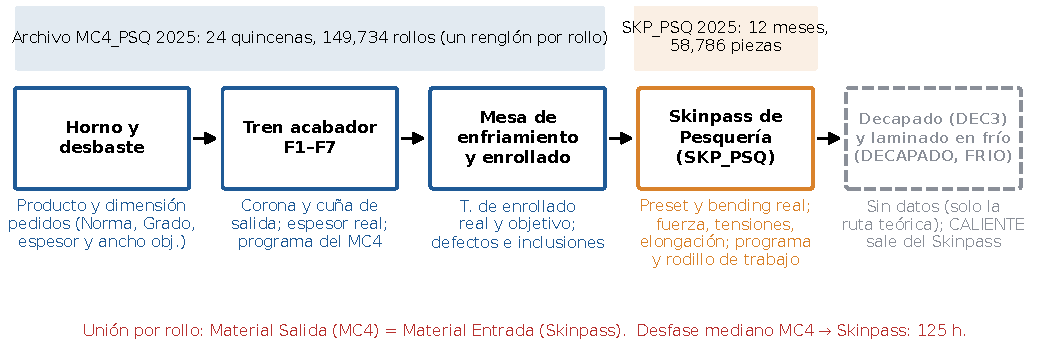
\includegraphics[width=\textwidth]{figuras/mapa_proceso.pdf}
\caption{\textbf{Cada rollo del MC4 llega al Skinpass varios días después, y sus dos registros se ligan rollo por
rollo.} Pregunta que responde: ¿en qué etapa nace cada dato que usamos? Se lee de izquierda a derecha, en el orden
en que viaja el acero. Bajo cada etapa están los datos que usamos (azul: archivo del MC4; naranja: archivo del
Skinpass). El decapado y la laminación en frío van después del Skinpass y no tienen datos.}
\label{fig:mapa}
\end{figure*}

Usamos dos fuentes de Ternium para todo 2025 (Fig.~\ref{fig:mapa}). La primera son 24 archivos quincenales del MC4
con un renglón por rollo (\NRollosMC{} rollos, 280 columnas): especificación del pedido, temperaturas, perfil de salida
y defectos. La segunda son 12 archivos mensuales del Skinpass de Pesquería con un renglón por pieza procesada
(\NRegistrosSKP{} registros, 208 columnas): programa, rodillo de trabajo, modo del molino, preset y valor real
promedio de bending, fuerza y tensiones, elongación, dictamen y defectos. La llave de unión es el identificador de
salida del MC4, que el Skinpass registra como material de entrada. Un rollo puede salir del Skinpass en varias piezas
(\NRollosDivididos{} rollos, \PctDivididos\,\%); las variables numéricas se agregan por rollo como promedio ponderado
por el peso de cada pieza, las banderas como ``alguna pieza'' y el programa, la fecha y el rodillo son los de la
primera pieza (las piezas comparten programa en todos los casos salvo uno). No ligan \NRegistrosSinLiga{} registros
del Skinpass, en su mayoría reprocesos de piezas ya pasadas y rollos laminados a fines de 2024; se cuentan por motivo
en el repositorio y se excluyen.

\subsection{Población y unidad de análisis}
\label{sec:poblacion}

\begin{table}[t]
\centering
\caption{Población de estudio paso a paso. Cada paso conserva los rollos que cumplen su criterio y los anteriores.
Progr.~SKP: programas del Skinpass distintos.}
\label{tab:poblacion}
\footnotesize
\begin{tabular}{cL{3.15cm}rrr}
\toprule
Paso & Criterio & Rollos & Excluidos & Progr. SKP \\
\midrule
0 & Rollos del MC4 en 2025 & 149,734 & -- & -- \\
1 & Ruta teórica con SKP\_PSQ (cualquier forma final) & 50,016 & 99,718 & -- \\
2 & Con registro en el Skinpass 2025 & 47,410 & 2,606 & 858 \\
3 & Laminados antes del 1-dic-2025 (censura) & 44,313 & 3,097 & 831 \\
4 & Con bending real y preset (Y definido) & 44,272 & 41 & 831 \\
5 & Además con corona relativa válida & 43,208 & 1,064 & 831 \\
\bottomrule
\end{tabular}

\end{table}

La Tabla~\ref{tab:poblacion} muestra cuántos rollos quedan en cada paso. Incluimos los rollos de \emph{cualquier}
forma final con el Skinpass de Pesquería en su ruta teórica, incluidos los \NOtras{} de formas finales que no terminan
en ``SKP'' y que la Entrega~I había excluido sin justificación: pasan por el Skinpass en la misma proporción
(\PctOtrasEnSKP\,\%) que los de forma final caliente (\PctCalienteEnSKP\,\%) o decapada (\PctDecapadoEnSKP\,\%).
Cortamos en los rollos laminados antes del 1 de diciembre porque solo \PctDicEnSKP\,\% de los de diciembre aparece en
el Skinpass de 2025; el resto se procesó en enero de 2026. Los excluidos por ese corte no son como los demás (corona
relativa mediana de \CoronaRelMedianaDic\,\% contra \CoronaRelMediana\,\%), así que el corte entra en el análisis de
robustez. Los \NExclSinCorona{} rollos sin corona válida quedan fuera solo de la asociación; casi todos fueron
retenidos en el MC4 (\PctRetenidoSinCorona\,\%, porque la regla de ``mal perfil'' se activa cuando falta la corona),
pero su corrección mediana es parecida a la del resto (\YMedianaSinCorona{} contra \YMediana~kN): la exclusión no depende
del resultado.

La unidad de análisis es el rollo del MC4, y siempre reportamos rollos y programas del Skinpass (\NProgramas{}
programas, con mediana de \MedianaRollosPrograma{} rollos). El \emph{producto} es la combinación de norma y grado
(\NProductos{} productos); la \emph{dimensión}, el rango de espesor objetivo por el rango de ancho objetivo del pedido
(valores especificados, no medidos); el \emph{tipo de material}, caliente, decapado o frío. Llamamos \emph{celda} a
cada combinación de producto, dimensión y mes (\NCeldas{} celdas).

\subsection{Resultado y variables que no pueden explicarlo}
\label{sec:resultado}
El resultado principal es la corrección de bending,
\begin{equation}
\Y_i = B^{\mathrm{real}}_i - B^{\mathrm{preset}}_i \quad [\mathrm{kN}],
\label{eq:y}
\end{equation}
la diferencia entre el bending real promedio del rollo y el preset de la receta. Es lo que el lazo de control ajustó
más allá de lo que fijó la receta: si el preset anticipara lo que el rollo necesita, $\Y$ sería cero. En la población,
$\Y$ tiene mediana de \YMediana~kN y desviación estándar de \YDE~kN. Como indicadores secundarios reportamos el
bending real (que no depende de las unidades del preset), el porcentaje de rollos con un defecto registrado por un
inspector en el Skinpass (\PctDefInspector\,\%), el porcentaje de rollos retenidos en el Skinpass (\PctRetenido\,\%)
y la elongación lograda en los rollos procesados en modo de elongación (\PctModoElongacion\,\% de la población).
Descartamos como resultados las etiquetas que el sistema genera por regla (por ejemplo, el defecto de espesor del
Skinpass, que se activa por el diámetro del rollo) y los dictámenes de ambos molinos, que son posteriores al
resultado. Por la misma razón, el preset no puede usarse como variable explicativa (es un componente de $\Y$), ni la
fuerza, las tensiones o la elongación reales, que el mismo proceso genera junto con el bending.

\subsection{Diagrama causal y conjunto de ajuste}
\label{sec:diagrama}

\begin{figure*}[t]
\centering
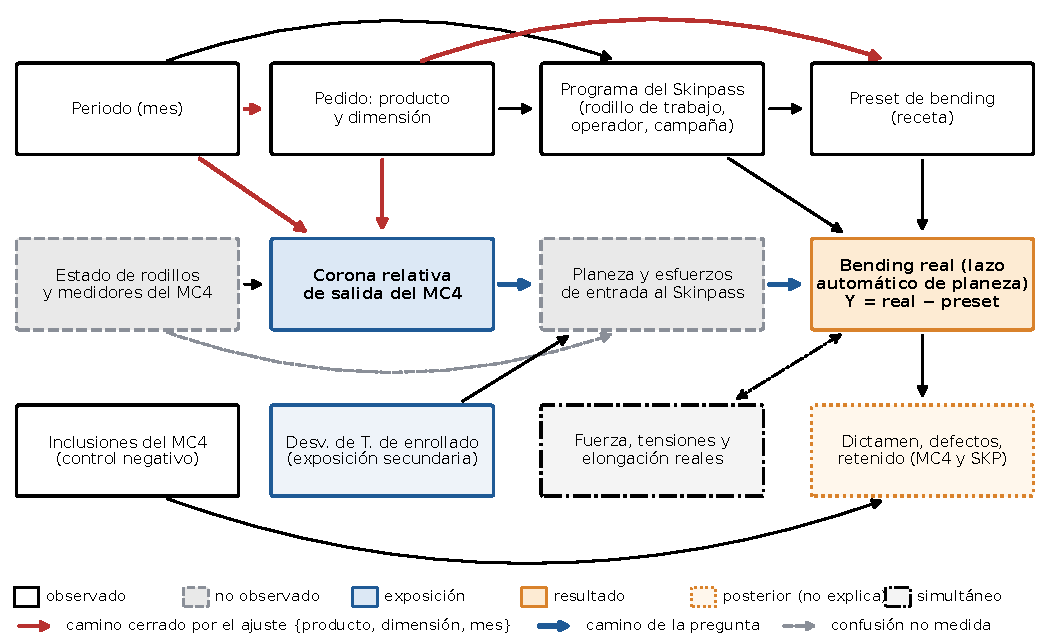
\includegraphics[width=\textwidth]{figuras/diagrama_causal.pdf}
\caption{\textbf{Ajustar por producto, dimensión y mes cierra los caminos de confusión observados entre la corona del
MC4 y la corrección de bending; la planeza de entrada y el estado de los rodillos quedan sin medir.} Pregunta que
responde: ¿qué hay que ajustar para comparar rollos con distinta corona, y qué no podemos ver? Cada flecha dice ``esto
influye en aquello''. Respecto a la Entrega~I se agregan el periodo, el programa del Skinpass, el preset dentro de un
lazo cerrado y la planeza de entrada, y se corrige el orden: el Skinpass va antes del decapado.}
\label{fig:dag}
\end{figure*}

La Fig.~\ref{fig:dag} resume lo que sabemos del proceso. El pedido (producto y dimensión) fija la corona que
el MC4 apunta a entregar y la receta del Skinpass; el periodo cambia la mezcla de pedidos, el estado del molino y de
sus medidores, y la programación. Esos dos caminos (en rojo) hacen que, sin ajuste, comparar rollos con distinta corona
sea comparar pedidos y meses distintos. El conjunto de ajuste que se desprende del diagrama es, por eso,
\{producto, dimensión, mes\}, que implementamos como efectos fijos de celda. El programa del Skinpass influye en el
preset y en el bending real pero no en la corona con que el rollo sale del MC4, de modo que no confunde la asociación
corona~$\rightarrow$~$\Y$: lo usamos para agrupar la incertidumbre y como fuente de variación en la descomposición, no
como ajuste. Quedan sin medir la planeza de entrada al Skinpass, el estado de los rodillos de ambos molinos y las
decisiones del operador; la sección~\ref{sec:validacion} acota cuánto podrían cambiar la conclusión. La
Tabla~\ref{tab:variables} resume el papel de cada variable.

\begin{table*}[t]
\centering
\caption{Variables y sus papeles en el diagrama causal. ``Ajuste'' indica si la variable entra al conjunto de ajuste
de la asociación corona~$\rightarrow$~$\Y$.}
\label{tab:variables}
\footnotesize
\begin{tabular}{L{3.6cm}L{4.1cm}L{1.6cm}L{6.9cm}}
\toprule
Variable & Papel en el diagrama & Ajuste & Por qué \\
\midrule
Producto, dimensión & Confusor (el pedido fija la corona y la receta) & Sí & Abre los caminos pedido $\rightarrow$ corona y pedido $\rightarrow$ preset \\
Mes & Confusor (mezcla de pedidos, estado de medidores) & Sí & La corona y la corrección cambian durante el año \\
Programa del Skinpass & Fuente de variación de $\Y$ & No (agrupa errores) & No causa la corona; se usa en la descomposición y para agrupar la incertidumbre \\
Corona relativa del MC4 & Exposición principal & --- & Corona / espesor, en puntos porcentuales; continua, sin cortes convencionales \\
Desv. de T. de enrollado & Exposición secundaria & --- & Real menos objetivo (°C) \\
Preset de bending & Componente de $\Y$ & No & Usarlo como explicativa crea un acoplamiento mecánico con $\Y$ \\
Fuerza, tensiones y elongación reales & Respuestas simultáneas & No & Se generan en el mismo proceso que $\Y$ \\
Dictamen, defectos, retención & Posteriores al resultado & No & Etiquetas derivadas, en buena parte por regla \\
Inclusiones del MC4 & Control negativo & No & Nacen en el acero, aguas arriba; no deberían responder al Skinpass \\
Acuñamiento (cuña) & Comprobación & Solo en R7 & Ternium indicó que no es prioritario \\
\bottomrule
\end{tabular}
\end{table*}

La exposición principal es la corona relativa, la corona de salida dividida entre el espesor y expresada en puntos
porcentuales (pp) del espesor (mediana \CoronaRelMediana\,\%), como variable continua, sin los cortes convencionales
de la Entrega~I. La cuña sale de la pregunta: Ternium indicó que no es prioritaria y en la exploración no se asoció
con la corrección de forma consistente; se conserva solo como comprobación. Seis supuestos sobre el significado de las
columnas, que ya no podemos confirmar con el Socio Formador, se escriben con su evidencia y su prueba de sensibilidad
en el Anexo~\ref{sec:anexo-supuestos}; los dos más importantes son que el preset está en kN como el bending real y que
un preset de cero significa ``sin preset'' (\PctPresetCero\,\% de los rollos).

\subsection{Análisis}
\label{sec:analisis}

\paragraph{Soporte} Antes de estimar, contamos por producto los rollos, programas, meses y celdas con al menos cinco
rollos, y la variación de la corona relativa dentro de celda. Un producto sin variación de corona dentro de celda no
aporta a la asociación y sale con nota.

\paragraph{Descomposición} Para cada nivel $\ell$ de la jerarquía tipo~$\rightarrow$~producto~$\rightarrow$~dimensión
$\rightarrow$~programa~$\rightarrow$~rollo calculamos la fracción de la suma de cuadrados de $\Y$ que explica,
\begin{equation}
f_\ell = \frac{\sum_i \left(\bar{\Y}_{c_\ell(i)} - \bar{\Y}_{c_{\ell-1}(i)}\right)^2}{\sum_i \left(\Y_i - \bar{\Y}\right)^2},
\label{eq:descomp}
\end{equation}
donde $c_\ell(i)$ es la celda del rollo $i$ en el nivel $\ell$. Con grupos pequeños cualquier agrupación parece explicar
mucho, así que cada fracción se compara con la que daría el azar, permutando 100 veces las etiquetas del nivel dentro de
su celda padre; reportamos el \emph{exceso sobre el azar}, $f_\ell$ menos la media nula. Su intervalo de 95\,\% se
obtiene de 200 réplicas en las que se toma al azar la mitad de los programas, sin reemplazo. Elegimos este método en
lugar del bootstrap con reemplazo porque duplicar programas sesga las fracciones de suma de cuadrados (bitácora del
plan). La descomposición se repite con el programa antes que el producto, para mostrar cuánto depende del orden, y
con el día, la semana y el rodillo de trabajo en lugar del programa.

\paragraph{Asociación} Estimamos
\begin{equation}
\Y_i = \beta\, \mathrm{corona}_i + \gamma\, \Delta T_i + \alpha_{c(i)} + \varepsilon_i ,
\label{eq:fe}
\end{equation}
con efectos fijos $\alpha_c$ de celda, la desviación de la temperatura de enrollado $\Delta T_i$ como exposición
secundaria y errores agrupados por programa del Skinpass, con corrección CR1 que cuenta los efectos fijos
absorbidos~\cite{cameron2015}. Reportamos $\beta$ en kN por punto porcentual de corona relativa y por una desviación
estándar de la corona dentro de celda, su $R^2$ parcial y la curva de $\Y$ por deciles de la corona, ambas centradas en
su celda. La misma especificación, con el preset como resultado, comprueba que la receta no reacciona a la corona del
rollo. Para la heterogeneidad estimamos la misma pendiente dentro de cada producto con al menos 300 rollos (efectos fijos
de dimensión por mes) y controlamos la tasa de descubrimientos falsos~\cite{benjamini1995}.

\paragraph{Predicción} Para saber si la información previa al Skinpass permite \emph{anticipar} $\Y$, comparamos un
solo modelo de aprendizaje automático, \emph{gradient boosting} con producto, dimensión, tipo, mes, corona relativa,
desviación de temperatura de enrollado y objetivos de espesor, ancho y temperatura, contra una línea base sencilla: la
media de $\Y$ por producto y dimensión en entrenamiento, que es lo que haría una receta por producto. Ambos se evalúan
con la misma validación: cinco particiones agrupadas por programa (ningún programa queda dividido) y una partición
temporal (entrenar con los programas de enero a agosto y evaluar de septiembre a noviembre)~\cite{roberts2017}. Una
validación aleatoria se reporta solo para mostrar cuánto infla el desempeño mezclar rollos de un mismo programa. Los
hiperparámetros se eligen dentro de cada partición de entrenamiento. Antes de correr el modelo fijamos qué cuenta como
mejora clara: bajar el error absoluto medio (MAE) en las cinco particiones agrupadas y en la temporal. La importancia de
cada variable, por permutación, describe lo que el modelo usa para predecir y no un efecto~\cite{shmueli2010}.

\subsection{Validación y sensibilidad}
\label{sec:validacion}
Sin verdad de terreno, sometimos la asociación a cuatro anclajes, cada uno con lo que la habría refutado, escrito antes
de verlo. \textbf{V1, control negativo}~\cite{lipsitch2010}: las inclusiones del MC4 nacen en el acero y no deberían
asociarse con $\Y$; habría refutado la conclusión una asociación con intervalo que excluya cero y magnitud comparable a
la de la corona. \textbf{V2, consistencia física}: una banda con más corona relativa necesita un claro entre rodillos
más abierto al centro, y el doblado positivo de los rodillos de trabajo cierra el centro, de modo que el lazo debería
responder con un bending más negativo; este argumento mecánico es nuestro (la literatura revisada no fija el signo), y
lo habría refutado una pendiente positiva con intervalo que excluya cero. \textbf{V3, robustez}~\cite{steegen2016}:
nueve decisiones de depuración razonables (R1~umbral de corona imposible; R2~definición de producto; R3~corte de
censura; R4~rollos divididos; R5~preset cero; R6~rollos sin el Skinpass en la ruta; R7~cuña como covariable; R8~presets
mayores que el máximo bending real; R9~rodillo de trabajo en lugar de programa), mostradas juntas; la habría refutado un
cambio de signo de la pendiente o que el producto superara al programa. \textbf{V4, programa contra periodo}: sustituir
el programa por el día o la semana; no refuta, pero si da lo mismo hay que escribir ``programa o periodo''. Para la
confusión no medida reportamos el valor de robustez de Cinelli y Hazlett~\cite{cinelli2020}, la proporción de la
varianza residual de la exposición y del resultado que un confusor tendría que explicar para anular la pendiente, y lo
comparamos con el del producto como confusor observado de referencia. Todos los contrastes examinados (\NContrastes)
están en la tabla completa del repositorio (Anexo~\ref{sec:anexo-contrastes}).
